% !TEX program = xelatex

\documentclass[a4paper,11pt]{article}

\usepackage{latex_style}
\DeclareMathOperator{\sech}{sech}

\DeclareMathOperator{\sn}{sn}
\DeclareMathOperator{\cn}{cn}
\DeclareMathOperator{\dn}{dn}

\title{Gauss maps of Delaunay Surfaces and their Spectral Curves}
\author{Ross Ogilvie}
\date{June 2017}

\begin{document}
\maketitle

\section*{Cheatsheet for Elliptic Functions}
The basic Jacobi elliptic functions are $\sn(z;k)$, $\cn(z;k)$ and $dn(z;k)$, which are functions of $z\in\C$ and the elliptic modulus $k\in(0,1)$. For us, $k$ will be parameterising the family of Delaunay surfaces and so be a constant on each surface. It is common to omit this argument. They obey the following trigonmetric type relations
\[
\sn^2 z + \cn^2 z = 1,\;\;\; k^2 \sn^2 z  + \dn^2 z = 1.
\]
They have the following values at zero
\[
\sn 0 = 0, \;\;\; \cn 0 = 1, \;\;\; \dn 0 = 1.
\]
They differentiate in the following ways
\[
\frac{d}{dz}\sn z = \cn z \dn z, \;\;\;
\frac{d}{dz}\cn z = -\sn z \dn z, \;\;\;
\frac{d}{dz}\dn z = -k^2\sn z \cn z.
\]
In the limit as the elliptic modulus goes to $0$ and $1$ these functions degenerate to the following elementary functions
\begin{align*}
\sn(z;0) &= \sin z & \sn(z;1) &= \tanh z \\
\cn(z;0) &= \cos z & \cn(z;1) &= \sech z \\
\dn(z;0) &= 1 & \dn(z;1) &= \sech z
\end{align*}











\section*{Roadmap}

Before we launch into calculation, let us give a roadmap to the spectral curve. The first step is to construct the family of flat connections from the harmonic map $N$. Given $N$, we will pull back the Mauer-Cartan form $N^{-1}dN$. This is useful, because we need the pullback of the Levi-Civitia connection $d_{LC}$, and by Lie group theory this is given as the average of the left and right connections. The difference of the left and right connections ($d_L$ and $d_R$ respectively) is exactly the Mauer-Cartan form, hence
\[
d_{LC} = d_L + \frac{1}{2}N^{-1}dN.
\]
The left gauge is useful because it is straightforward to do explicit calculations in. The Mauer-Cartan form is also used to define the Higgs field $Φ$. It is the $(1,0)$ part of half the Mauer-Cartan form, and as $N^{-1}dN$ is $\su_2$-valued
\[
2(Φ- Φ^*) = N^{-1}dN.
\]
The family of flat connections, indexed by $ζ\in\C^\times$, is given by 
\begin{align*}
d_ζ 
:=& d_{LC} + ζ^{-1}Φ - ζΦ^* \\
=& d_L + Φ - Φ^* + ζ^{-1}Φ - ζΦ^* \\
=& d_L + (1+ζ^{-1})Φ - (1+ζ)Φ^*.
\labelthis{eqn:connections}
\end{align*}
Once we have this family of connections, we may take a pair of basis loops for the fundamental group and consider the holonomy $H(ζ)$ and $\tilde{H}(ζ)$ of $d_ζ$. Because the fundamental group of the torus is abelian, these matrices commute and therefore share eigenspaces. Thus we may define the spectral curve as the closure of 
\[
\{ (ζ,L) \in \C^\times \times \CP^1 | L \text{ is an eigenline of } H(ζ) \}.
\]

In the specific case of the unduloid and nodoid, we may save ourselves some effort and shortcut our way to the spectral curve. Because the spectral genus is low, it is not possible for the spectral curves to have singularities and so we just need to find the branch points, not their orders. In the language of eigenlines, this is just saying the two eigenlines can only coincide to first order. At such points there is a single eigenvalue of $H(ζ)$.

The second simplification we will leverage is the rotational symmetry. This means there will be a gauge transformation that makes the connection matrix constant in the rotation coordinate $v$. If the coordinate along the axis is $t$, then we will be able to write the family of connections as
\[
d_ζ = d - B(t,ζ).
\]
Taking the loop $v\in [0,2π]$ and $t=0$, the corresponding holonomy matrix will be
\[
H(ζ) = \exp 2π B(0,ζ).
\]
Our ability to write the holonomy as a matrix exponential corresponds to the existence of an exact differential in the case of an elliptic spectral curve. The eigenvalues of $H(ζ)$ will coincide exactly when the eigenvalues $\pm μ(ζ)$ of $B(0,ζ)$ do, and as $B$ is $\su_2$
\[
μ^2(ζ) = - \det B(0,ζ).
\] 
In summary, the branch points of the spectral curve are the values of $ζ$ for which the determinant of $B(0,ζ)$ vanishes.













\section*{Unduloid}
A surface of revolution has the following form
\[
f(v,t) = (φ(t) \cos v, φ(t) \sin v, ψ(t)).
\]
Its Gauss map is then
\[
N(v,t) = \frac{1}{φ} (-φ', ψ' \sin v, ψ' \cos v).
\]
For the unduloid, these functions are given by
\begin{align*}
φ(t) &= \dn t + k \cn t \\
φ'(t) &= -k^2\sn t\cn t - k \sn t \dn t = -k φ(t) \sn t \\
ψ'(t) &= (\dn t + k \cn t) \dn t = φ(t) \dn t.
\end{align*}
(These formulae come from \cite{Mladenov2014}. There are many parameterisations of the Delaunay surfaces floating around online, but rarely are they conformal or written with standard elliptic functions; this source has both).
This gives the Gauss map as
\[
N(v,t) = (k \sn t, \dn t \sin v, \dn t \cos v).
\labelthis{eqn:unduloid}
\]
If we embed this into $\S^3 = \SU(2)$ such that the $(0,0)$ is mapped to the identity matrix, one option is
\[
N(v + \iu t)
= \begin{bmatrix}
\dn t \cos v & -k \sn t + \iu \dn t \sin v \\
k \sn t + \iu \dn t \sin v & \dn t \cos v
\end{bmatrix}.
\]
Any other option will be a rotation of this one and so will produce the same spectral data. The Mauer-Cartan form is 
\begin{align*}
N^{-1}dN
&= \begin{bmatrix}
\iu k \sn t \dn t \cos v & -k \sn t \dn t \sin v + \iu \dn^2 t \\
k \sn t \dn t \sin v + \iu \dn^2 t & -\iu k \sn t \dn t \cos v
\end{bmatrix} dv \\
&\qquad\qquad + \begin{bmatrix}
-\iu k \cn t \sin v & -k \cn t \cos v \\
k \cn t \cos v & \iu k \cn t \sin v
\end{bmatrix} dt
\\
&= k \sn t \dn t \begin{bmatrix}
\iu \cos v & -\sin v \\
\sin v & -\iu \cos v
\end{bmatrix} dv
+ \dn^2 t \begin{bmatrix}
0 & \iu \\
\iu & 0
\end{bmatrix} dv \\
&\qquad\qquad + k \cn t \begin{bmatrix}
-\iu \sin v & -\cos v \\
\cos v & \iu \sin v
\end{bmatrix} dt.
\end{align*}
Because the map is has a rotational symmetry in $v$, there should be a gauge such that the connection matrix is constant in $v$. Indeed, let
\[
h = \frac{1}{\sqrt{2}}\begin{bmatrix}
\sqrt{1-\sin v} & -\iu \sqrt{1+\sin v} \\
-\iu \sqrt{1+\sin v} & \sqrt{1-\sin v}
\end{bmatrix},
\]
then
\[
h^{-1}N^{-1}dN h
= k \sn t \dn t \begin{bmatrix}
0 & 1 \\
-1 & 0
\end{bmatrix} dv
+ \dn^2 t \begin{bmatrix}
0 & \iu \\
\iu & 0
\end{bmatrix} dv 
+ k \cn t \begin{bmatrix}
\iu & 0 \\
0 & -\iu
\end{bmatrix} dt.
\]
If a connection matrix is $A$, then the connection matrix in the new gauge is $h^{-1}dh + h^{-1}Ah$. Let us then calculate
\[
h^{-1} dh = \frac{1}{2}\begin{bmatrix}
0 & \iu \\ \iu & 0
\end{bmatrix} dv.
\]
Following Hitchin, we define the Higgs field $Φ$ to be half the $(1,0)$ part of the Mauer-Cartan form. The conformal type of the domain torus is given by $z = v+\iu t$, so 
\[
dv = \frac{1}{2}(dz + d\bar{z}),\;\;\;
dt = \frac{-\iu}{2}(dz - d\bar{z}).
\]
Thus in the present gauge
\[
Φ
= \frac{1}{4}k \sn t \dn t \begin{bmatrix}
0 & 1 \\
-1 & 0
\end{bmatrix}
+ \frac{1}{4}\dn^2 t \begin{bmatrix}
0 & \iu \\
\iu & 0
\end{bmatrix}
+ \frac{1}{4}k \cn t \begin{bmatrix}
1 & 0 \\
0 & -1
\end{bmatrix} \;dz.
\]
Recall from the roadmap above that we can find the spectral curve if we find the roots of $\det B(0,ζ)$, where $B$ is the connection matrix of this family. From \eqref{eqn:connections}
\begin{align*}
d_ζ 
&= d_L + (1+ζ^{-1})Φ - (1+ζ)Φ^* \\
&= d + h^{-1}dh + (1+ζ^{-1})Φ - (1+ζ)Φ^*.
\end{align*}
Assembling all the pieces
\begin{align*}
\det B 
&= \det \left\{ \frac{1}{2}\begin{bmatrix}
0 & \iu \\ \iu & 0
\end{bmatrix} 
- \frac{1}{4} (1+ζ^{-1}) \begin{bmatrix}
k & \iu \\
\iu & -k
\end{bmatrix}
+ \frac{1}{4} (1+ζ) \begin{bmatrix}
k & -\iu \\
-\iu & -k
\end{bmatrix} \right\} \\
%%%%%%%%%%%%%%%%
&= \frac{1}{16}ζ^{-2}\det \begin{bmatrix}
kζ^2 - k & -\iu (ζ^2+1) \\
-\iu (ζ^2+1) & -(kζ^2 - k)
\end{bmatrix} \\
%%%%%%%%%%%%%%%%
&= \frac{1}{16}ζ^{-2} \left[ (kζ^2 - k)^2 - (ζ^1 + 1)^2 \right] \\
&= \frac{1}{16}ζ^{-2} \left[ (kζ^2 - k) - (ζ^1 + 1) \right]\left[ (kζ^2 - k) + (ζ^1 + 1) \right] \\
&= -\frac{1}{16}(1-k^2)ζ^{-2} \left( ζ^2 + \tilde{k}^2 \right)\left( ζ^2 + \tilde{k}^{-2} \right),
\end{align*}
where
\[
\tilde{k}^2 = \frac{1-k}{1+k}.
\]
Thus the roots of the spectral curve are 
\[
ζ = \pm \iu\tilde{k}, \pm \iu \tilde{k}^{-1}.
\]









\section*{Nodoid}
This section exactly parallels the previous one, so I will omit repeating the commentary and provide formula for those playing at home to use as checkpoints. In the notation of the previous section, for the nodoid
\begin{align*}
φ(t) &= \dn (t/k) + k \cn (t/k) \\
φ'(t) &= -\sn (t/k)\dn (t/k) - k \sn (t/k) \cn (t/k) = - φ(t) \sn (t/k) \\
ψ'(t) &= (\dn (t/k) + k \cn (t/k)) \dn (t/k) = φ(t) \dn (t/k).
\end{align*}
This gives the Gauss map as
\[
N(v + \iu t)
= \begin{bmatrix}
\cn (t/k) \cos v & \sn (t/k) + \iu \cn (t/k) \sin v \\
-\sn (t/k) + \iu \cn (t/k) \sin v & \cn (t/k) \cos v
\end{bmatrix}.
\labelthis{eqn:nodoid}
\]
The Mauer-Cartan form is 
\begin{align*}
N^{-1}dN
&= - \sn (t/k) \cn (t/k) \begin{bmatrix}
\iu \cos v & -\sin v \\
\sin v & -\iu \cos v
\end{bmatrix} dv
+ \cn^2 (t/k) \begin{bmatrix}
0 & \iu \\
\iu & 0
\end{bmatrix} dv \\
&\qquad\qquad - \frac{\dn (t/k)}{k} \begin{bmatrix}
-\iu \sin v & -\cos v \\
\cos v & \iu \sin v
\end{bmatrix} dt.
\end{align*}
These matrices are exactly the same as for the unduloid, and so in particular we may use the same gauge transformation to make them constant in $v$. The Higgs field is now
\[
Φ
= - \frac{1}{4} \sn (t/k) \cn (t/k) \begin{bmatrix}
0 & 1 \\
-1 & 0
\end{bmatrix}
+ \frac{1}{4}\cn^2 (t/k) \begin{bmatrix}
0 & \iu \\
\iu & 0
\end{bmatrix}
- \frac{1}{4}\frac{\dn (t/k)}{k} \begin{bmatrix}
1 & 0 \\
0 & -1
\end{bmatrix} \;dz.
\]
This time, the determinant of the connection matrix along the loop where $t=0$ is 
\begin{align*}
\det B 
%%%%%%%%%%%%%%%%
&= \frac{1}{16}k^{-2}ζ^{-2}\det \begin{bmatrix}
ζ^2 - 1 & \iu k (ζ^2+1) \\
\iu k (ζ^2+1) & -(ζ^2 - 1)
\end{bmatrix}  \\
%%%%%%%%%%%%%%%%
&= \frac{1}{16}k^{-2}(1-k^2)ζ^{-2} \left( ζ^2 - \tilde{k}^2 \right)\left( ζ^2 - \tilde{k}^{-2} \right),
\end{align*}
where again we define
\[
\tilde{k}^2 = \frac{1-k}{1+k}.
\]
Thus the roots of the spectral curve are 
\[
ζ = \pm \tilde{k}, \pm \tilde{k}^{-1}.
\]

\section*{Discussion}
The first thing to note is that the second part of the argument given in \cite{Hitchin1990}[p692] seems only to apply to the unduloids and not the nodoids, but as I don't understand the argument I can't comment as to why. The first part of the argument, which uses the reflectional symmetry about a meridian of the Delaunay surface to show that the branch points must satisfy $α = \pm \bar{α}$ is shown explictly by the above.

The elliptic modulus $k$ acts as a parameter for both families of surfaces. As $k$ runs from $0$ to $1$, $\tilde{k}$ runs from $1$ down to $0$. For both families, as $k$ tends to $1$, the branch points inside the unit circle tend to the origin, whereas as $k$ tends to $0$ they coalesce on the unit circle. The common $k=1$ limit represents the transition from unduloid to nodoid through the chain of spheres. We may set $k=1$ in either formula for $N$, equations \eqref{eqn:unduloid} or \eqref{eqn:nodoid}, to get
\[
N_{k=1} = \left( \tanh t, \sech t \sin v, \sech t \cos v \right),
\]
written here as a map to $\R^3$ rather than some $2$-sphere inside $S^3$. This map covers the sphere except for the two points $(\pm 1, 0, 0)$, which are the limits as $t\to\pm\infty$. To understand this, it helps to look at the $z$ component of $N$ of the nodoid for $v=0$. This is the just function $\cn$.

\begin{center}
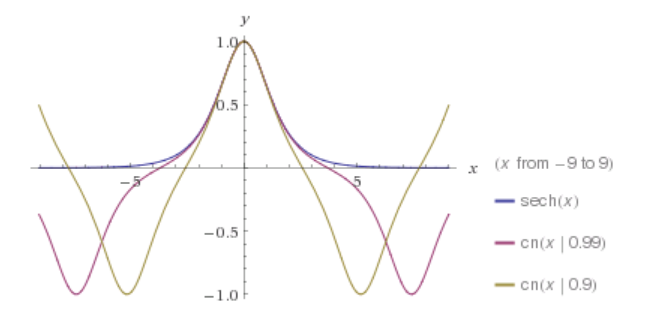
\includegraphics[width=\textwidth]{cn_plot.png}
\end{center}

For a nodoid, the normal starts pointing up, then as it goes to the looping bit its pointing down, and then as it comes to the next lobe its pointing up again. As $k$ tends to $1$, we see on the curve $\cn(x;0.99)$ above that it takes longer before it arrives at the next lobe (it, and in the limit it is unable to pass through the pinch.

Thus this map is not doubly periodic, and so not defined on a torus. This is expected, as a condition on the spectral curve is that it may not have singularities over $ζ=0$, and the curve that lies between the unduloids and nodoids is $η^2 = ζ^2$. However, this limiting $N_{k=1}$ is a map of the cylinder and so we should think about the spectral theory of maps of the cylinder. There is an interesting point here; one normally thinks of maps of the torus as sitting inside the space of maps of the cylinder by ignoring one of the periods. This example shows that that inclusion is not closed, and that maps of the cylinder may be `close' to maps of torus in more ways than not closing up.

The next limit to consider is not as interesting. It is the case of the unduloids as $k$ goes to $0$. The limit of this family is the straight cylinder, and the Gauss map is a map to the circle. This however fits with our observations of spectral genus zero harmonic maps in the limit that the branch points come together on the unit circle; they are also maps to the circle.

Finally, we may consider the limit of the nodoid family as $k\to 0$. It is a sphere; as the loopy bits grow and the lobes are pushed together, the nodoid becomes a single sphere. But this is somehow not a good limit. Indeed, from equation \eqref{eqn:nodoid} for the Gauss map, we see that many of the functions have the parameter $t/k$, which speeds up in this limit. If one rescales the parameter though, say as $s = t/k$, then the limit is
\[
N = (\sin s, \cos s \sin v, \cos s \cos v),
\]
which is standard polar coordinates on the sphere. This morally mirrors what one sees in the spectral genus zero case as branch points move to the points $ζ = \pm 1$. In that case the image of the map is fixed, but if we write the domain as $\C/\langle 1, \iu r\rangle$, then $r \to 0$ in the limit. In the same way for the nodoid, if we do this reparameterisation of $t$ to preserve the image, the domain is 
\[
v+\iu s \in \C/ \langle 2π, \iu 2π/k\rangle,
\]
which is also collapsing.

An analogy could be the following. Consider a cylinder parameterised by
\[
f(t,v) = (\cos v, \sin v, kt).
\]
For $k$ positive and negative, the cylinder is parameterised in `opposite' directions. And in the middle of the family, when $k=0$, is a circle. But it's a little odd to think of this change as the cylinders collapsing into a circle and then expanding out the other way. The analogy would say that you have a nodoid in one direction, then a sphere in the middle of the family, then nodoids in opposite direction. 

\bibliographystyle{ross_bibsty}
\bibliography{zotero}
\end{document}
